\chapter{Расчет излучения источников}\label{radiation}
FAINA позволяет рассчитывать электромагнитное излучение от источников с заданными функциями распределения излучающих частиц и другими параметрами. Построены модели следующих типов излучения: синхротронного, обратного комптоновского рассеяния, пионного распада в результате свободно-свободного взаимодействия протонов и тормозного излучения.
\section{Функции распределения частиц}
Важнейшими исходными данными для расчета любого типа излучения является функция распределения излучающих частиц. В коде FAINA для представления распределений используется абстрактный класс ParticleDistribution и семейство наседованных от него классов, соответствующих различным конкретным реализациям. Класс ParticleDistribution имеет следующие доступные методы:
	\begin{table}[h!]
	\label{ParticleDistribution}
	\begin{center}
		\begin{small}
		\begin{tabularx}{\textwidth}{|X|X|}
			\hline
			\textbf{ParticleDistribution} & \\
			\hline
			distribution(const double\& energy, const double\& mu, const double\& phi) & возвращает функцию распределения от энергии, косинуса полярного угла и азимутального угла, нормированную на единицу \\
			\hline
			distributionNormalized(const double\& energy, const double\& mu, const double\& phi) & возвращает функцию распределения от энергии, косинуса полярного угла и азимутального угла, нормированную на концентрацию \\
			\hline
			getConcentration() & возвращает концентрацию частиц\\
			\hline
		\end{tabularx}
	    \end{small}
    	\caption{Публичные методы класса ParticleDistribution }
	\end{center}
\end{table}
Для вычисления излучения необходимо в первую очередь задать распределение излучающих частиц. Для это нужно создать объект из подходящего класса-наследника ParticleDistribution. Дерево наследования на две большие ветви - распределения фотонов, представленных абстрактным классом PhotonDistribution и распределения массивных частиц - MassiveParticleDistribution. Схема наследования этих классов представлена на рисунке \ref{particleDistribution0}. 
\begin{figure}
	\centering
	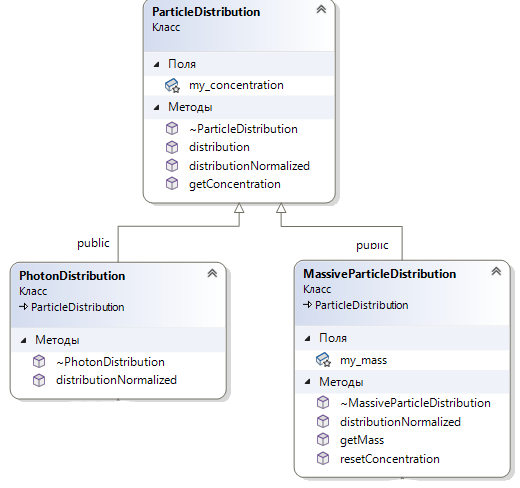
\includegraphics[width=10.5 cm]{./fig/particleDistribution0.png} 
	\caption{Схема наследования распределения фотонов и массивных частиц}
	\label{particleDistribution0}
\end{figure}
Важно отметить, что распределения фотонов не используются для представления результатов расчета излучения. Они нужны как входной параметр для расчета обратного комптоновского рассеяния. Класс PhotonDistribution не имеет дополнительных собственных методов и является лишь интерфейсом. Класс MassiveParticleDistribution тоже является абстрактным, в нем не задан конкретный вид распределения, но добавлены новые методы	\begin{table}[h!]
	\label{MassiveParticleDistribution}
	\begin{center}
		\begin{small}
			\begin{tabularx}{\textwidth}{|X|X|}
				\hline
				\textbf{MassiveParticleDistribution} & \\
				\hline
				getMass() & возвращает массу частиц \\
				\hline
				resetConcentration(const double\& n) & позволяет изменить полную концентрацию частиц\\
				\hline
			\end{tabularx}
		\end{small}
		\caption{Публичные методы класса MassiveParticleDistribution }
	\end{center}
\end{table}
\subsection{Распределения фотонов}

\subsection{Распределения массивных частиц}